\chapter{Билет №8}

\section*{Средства взаимодействия процессов — сокеты Беркли. Создание сокета — семейство, тип, протокол. Системный вызов sys\_socket() и struct socket. Состояния сокета. Адресация сокетов и ее особенности для разных типов сокетов. Модель клиент-сервер. Сетевые сокеты — сетевой стек, аппаратный и сетевой порядок байтов. Примеры реализации взаимодействия процессов по модели клиент-сервер с использованием сокетов и мультиплексированием (лаб. раб.).}

\section{Средства взаимодействия процессов — сокеты Беркли}
Сокеты -- универсальное средство взаимодействия параллельных процессов. Универсальность заключается в том, что сокеты используются как и на локальной машине, так и в распределенной системе (сети), в отличие от, например, разделяемой памяти, которая применима только на отдельно стоящей машине.

Распределенная система~---~система с раздельной памятью (объединенные в сеть компы с собственной памятью, в наших компах все ядра работают с общей памятью).

Сокет -- абстракция конечной точки соединения.

Взаимодействие на отдельной машине и в сети существенно разное: в сети это будет транспортный уровень (сетевой протокол, например, TCP/IP)

\begin{table}[H]
  \centering
  \begin{tabular}{p{1\linewidth}}
    \centering
    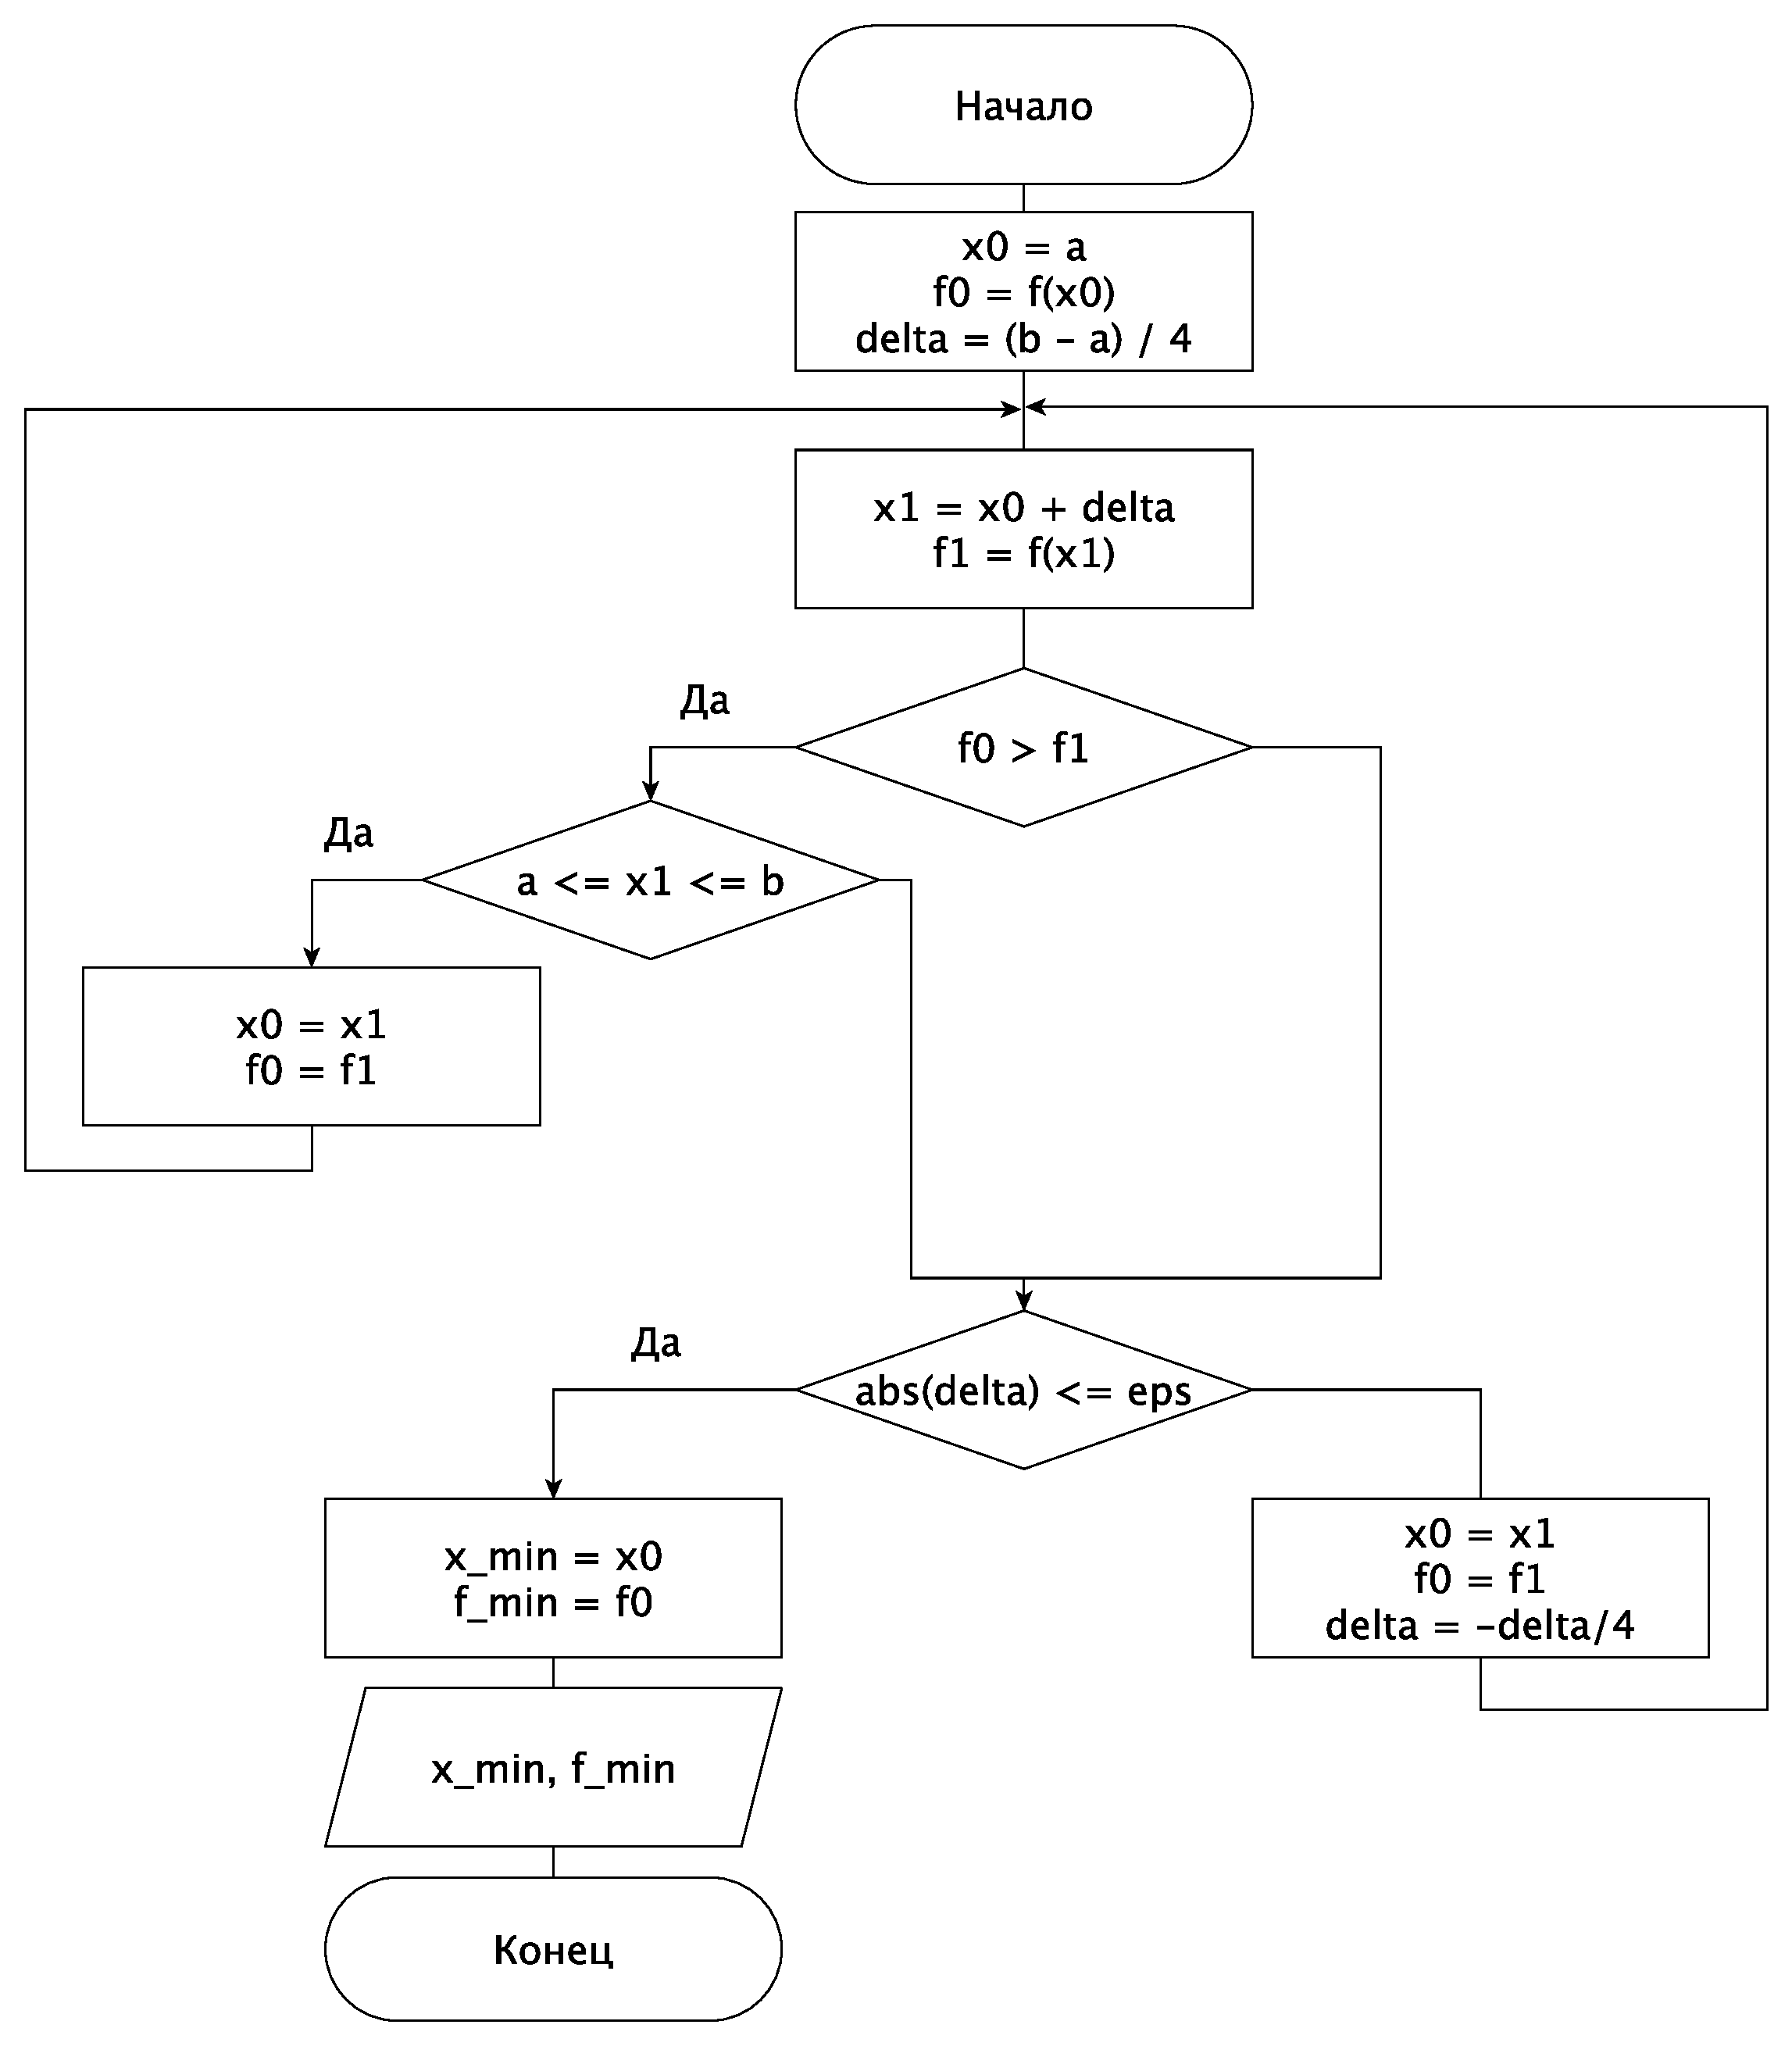
\includegraphics[width=0.8\linewidth]{./images/1.png}
  \end{tabular}
\end{table}

Парные сокеты обеспечивают дуплексную связь, т.е. сообщения можно передавать через один сокет в обе стороны (альтернатива pipe)

\begin{quote}
	\textbf{Парные сокеты vs программные каналы}

  Парные сокеты были созданы в UNIX BSD как универсальное (могут быть использованы для взаимодействяи параллельных процессов на отдельно стоящей машине и в распределенных системах) средство взаимодействия параллельных процессов.

  Распределенная система - у каждого узла (хоста) своя память.

  Отличия от pipe: парные сокеты обеспечивают дуплесную связь (двусторонюю, читение и запись), а pipe - симплексную (односторонюю)

  \textbf{BSD Сокеты}

  \begin{table}[H]
  \centering
  \begin{tabular}{p{1\linewidth}}
    \centering
    \includegraphics[width=0.8\linewidth]{./images/8-2.pdf}
  \end{tabular}
\end{table}

  Сокеты Packet созданы для непосредственного доступа приложений е сетевым устройстам

  Сокетов Netlink очень много, основные: NETLINK\_USERSOCK, NETLINK\_FIREWALL.

  Созданы для обмена данными между частями ядра и пространством пользователя.

  \textbf{Связь виртуальной файловой системы proc и сокетов NETLINK}

  В Linux есть ВФС proc, созданная специально для того, чтобы в пространстве пользователя можно было получить информацию о выполнении процессов. Но в ядре информации значительно больше (и о процессах, и о ресурсах). Очень важно иметь возможность получить ее. Ядро предоставляет средства для получения этой информации. Одним из таких средств являются сокеты NETLINK.
\end{quote}

\section{Создание сокета}

Сокеты для взаимодействия на отдельно стоящей машине/ в сети создаются системным вызовом

\begin{lstlisting}
int socket(int family, int type, int protocol);
\end{lstlisting}

\begin{quote}
\textit{Cинопсис~---~краткое описание. Не называть это сигнатурой!}
\end{quote}


Параметры системного вызова socket()

\begin{itemize}
\item family/domain - пространство имен
\begin{itemize}
\item AF\_UNIX - межпроцессорное взаимодействие на отдельно стоящей машине, часто говорят “домен UNIX”. Сокеты в файловом пространстве имен. 
\item AF\_INET - семейство TCP/IP для интернета версии 4 (IPv4). Интернет-домен, фактически любая компьютерная сеть
\item AF\_INET6 - семейство TCP/IP для IPv6
\item AF\_IPX - домен протокола IPX
\item AF\_UNSPEC - неопределенный домен
\end{itemize} 
AF - address family. Сокеты на отдельно стоящей машине (локальные сокеты) взаимодействуют через файловое пространство имен. Чтобы организовать взаимодействие процессов через сокеты AF\_UNIX, объявляется файл, который виден в файловой подсистеме как специальный файл (s - маленькая)
\begin{itemize}
\item SOCK\_STREAM - потоковые сокеты. Определяет ориентированное на потоки, надержное, упорядоченное, логическое соединение между двумя сокетами
\item SOCK\_DGRAM - опредялеют ненадежную службу дейтаграм без установления логического соединения, где пакеты модут передаваться без сохранения порядка (широковещательная передача данных)
\item SOCK\_RAW - низкоуровневые сокеты
\end{itemize}
\item protocol \\ 
обычно ставится 0 - протокол назначается по умолчанию. Например, для AF\_INET SOCK\_STREAM протокол TCP, для SOCK\_DGRAM это UDP, но можно задать протокол предописанной константой IPPROTO\_*, например, IPPROTO\_TCP
\end{itemize}

API~---~прикладной программный интерфейс, предоставляемый ОС (для программиста: набор функций, которые можно вызвать из приложения). Application Program Interface. API-функция => режим ядра (системный вызов).

\section{Системный вызок \\ sys\_socket()}
В ядре socket вызывает sys\_socket (листинг sys\_socket чуть ниже).

\begin{quote}
\textit{На лекциях не было, кусок кода ядра.}

\begin{lstlisting}
SYSCALL_DEFINE3(socket, int, family, int, type, int, protocol)
{
	return __sys_socket(family, type, protocol);
}
\end{lstlisting}
\end{quote}

\begin{lstlisting}
#include <net/socket.c>
asmlinkage long sys_socketcall(int call, unsigned long *args)
// ее текст = switch, переключающий ядро на разные функции, связанные с сокетом
{
  int err;
  if copy_from_user(a, args, nargs[call])
    return -EFAULT;
  a0 = a[0];
  a1 = a[1];
  switch(call)
  {
      case SYS_SOCKET: err= sys_socket(a0, a1, a[2]); break;
      case SYS_BIND: err= sys_bind(a0, (struct sockaddr*)a1, a[2]); break;
      case SYS_CONNECT: err= sys_connect(...); break;
      ...
      default: err = -EINVAL; break;
  }
  return err;
}
\end{lstlisting}
В switch перечисляются функии так называемого сетевого стека. Для них определены предописанные константы (макроопределения): (код с дефайнами относится к пояснению)

\begin{lstlisting}
<include/linux/net.h>
#define SYS_SOCKET 1
#define SYS_BIND 2
#define SYS_CONNECT 3
#define SYS_LISTEN 4
\end{lstlisting}

\begin{lstlisting}
asmlinage long sys_socket(int family, int type, int protocol)
{
  int retval;
  struct socket *sock;
  ...
  retval = sock_create(famaly, type, protocol, &sock);
  ...
  return retval;
}
\end{lstlisting}

\section{struct socket. Состояния сокета}
\begin{lstlisting}
struct socket // нет в 6 версии ядра
{
  socket_state state;
  short type;
  unsigned long flags;
  const struct proto_ops *ops;
  struct fasync_strcut *fasync_list;
  struct file *file;
  struct sock *sk;
  wait_queue_head_t wait;
}
\end{lstlisting}

flags - используется для синхронизации доступа.

struct proto\_ops - действия на сокете (protocol operations). Здесь можно зарегистрировать свои функции работы с сокетами.

У сокета различают 5 состояний, 4 из которых - стадии соединения:

\begin{itemize}
\item SS\_FREE - свободный сокет, с которым можно соединяться;
\item SS\_UNCONNECTED - несоединенный сокет;
\item SS\_CONNECTING - сокет находится в состоянии соединения;
\item SS\_CONNECTED - соединенный сокет;
\item SS\_DISCONNECTING - сокет разъединяется в данный момент.
\end{itemize}

Сокеты описываются как открытые файлы (они не хранятся во вторичной памяти, это файлы специального типа (сможем увидеть только в сокетах в файловом пространстве имент AF\_UNIX))

\section{Адресация сокетов и ее особенности для разных типов сокетов}

struct sockaddr - обращение к сокету выполняется по адресу (сокеты адресуются)

Взаимодействие на сокетах происходит по модели клиент-сервер

Адресация сокетов:
\begin{lstlisting}
struct sockaddr
{
  sa_family_t sa_family;
  char sa_data[14]; 
}
\end{lstlisting}
Такая структура адреса не подходит для интернета, так как там необходимо указывать номер порта и сетевой адрес. Для интернета разработана другая структура:

\begin{lstlisting}
struct soackaddr_in
{
  sa_family_t sa_family;
  unsigned short int sin_port;
  struct in_addr sin_addr;
  unsigned char sin_zero[sizeof(struct sockaddr) - sizeof(sa_family_t) - sizeof(uint16_t) - sizeof(struct in_addr)];
};
\end{lstlisting}

Сетевой адрес и номер порта должны быть указаны в сетевом порядке байтов.

\section{Аппаратный и сетевой порядок байтов}

Порядок байт:

\begin{itemize}
\item аппаратный
\item сетевой
\end{itemize}

Прямой и обратный порядок байт

  \begin{table}[H]
  \centering
  \begin{tabular}{p{1\linewidth}}
    \centering
    \includegraphics[width=0.8\linewidth]{./images/3.png}
  \end{tabular}
\end{table}

Сети оперируют портами и сетевыми адресами

\begin{lstlisting}
uint16_t htons(uint16_t hostint16) // host to network short
uint32_t htonl(uint32_t hostint32) // host to network long

uint16_t ntohs(uint16_t netshort); // network to host short
uint32_t ntohl(uint32_t netlong); // network to host long
\end{lstlisting}


\section{Модель клиент-сервер}
Взаимодействие на сокетах осуществляется по модели клиент-сервер: сервер предоставляет ресурсы и службы одному или нескольким клиентам, которые обращаются к серверу за обслуживанием. 

В момент, когда клиент запрашивает соединение с сервером, сервер может либо принять, либо отклонить запрос на соединение. Если соединение устанавливается, то оно поддерживается по определённому протоколу.
\section{Сетевой стек}

Сети ~ распределенные системы, т.е. у каждого хоста своя память

В сетях - только передача сообщений, которые должны сопровождаться адресом

Пакет - сообщение с адресом + служебная информация 

В Linux определен интерфейс между пользовательскими процессами и стеком сетевых протоколов в ядре.

\begin{quote}
Это не по семинару*

Модули протоколов группируются по семействам протоколов, такими, как AF\_INET, AF\_IPX и AF\_PACKET, и типам сокетов, такими, как \\ SOCK\_STREAM или SOCK\_DGRAM. Сетевой стек ядра Linux имеет две структуры:

struct socket — интерфейс высокого уровня, который используется для системных вызовов (именно поэтому он также имеет указатель struct file, который представляет файловый дескриптор)

struct sock — реализация в ядре для AF\_INET сокетов (есть также struct unix\_sock для AF\_UNIX сокетов, которые являются производными от данного), которые могут использоваться как в ядре, так и в режиме пользователя.
\end{quote}

\begin{table}[H]
  \centering
  \begin{tabular}{p{1\linewidth}}
    \centering
    \includegraphics[width=0.8\linewidth]{./images/4.pdf}
  \end{tabular}
\end{table}

socket() - создание точки соединения. Возвращает файловый дескриптор. Сокет - специальный файл (у него есть inode), назначение которого - обеспечивать соединения;

AF\_INET, SOCK\_STREAM - сетевое взаимодействие по протоколу TCP

bind() связывает сокет с адресом (сетевым (порт + API-адрес) в случае сокетов AF\_INET)

\begin{lstlisting}
int bind(int sockfd, struct sockaddr *addr, int addrlen);
\end{lstlisting}

struct sockaddr\_in - есть поле “порт” и “сетевой адрес” (у них должен быть сетевой порядок (применяем функцию htons())

На сервере вызов bind() обязателен, на клиенте нет, т.к. его точный адрес часто не играет никакой роли (если bind() не вызывается, адрес назначается клиентам автоматически)

listen() информаирует ОС о том, что он готов принимать соединения (имеет смысл только для протоколов, ориентированных на соединение (например, TCP)

\begin{lstlisting}
int listen(int sockfd, int baclog);
\end{lstlisting}
connect() - клиент устаналивает активное соединение с сокетом (с сервером)
\begin{lstlisting}
int connect(int sockfd, struct sockaddr *addr, int addrlen)
\end{lstlisting}

Для протокола без соединения (например, UDP) connect может использоваться для указания адреса назначения всех передаваемых пакетов

accept() - вызывается на стороне сервера, если соединение установлено. Сервер принимает соединение, *только если* он получил запрос на соединение.

\begin{lstlisting}
int accept(int sockfd, void* addr, int *addrlen)
\end{lstlisting}

Когда соединение принимается, accept()  создает копию исходого сокета, чтобы сервер мог принимать другие соединения. Исходный сокет остается в состоянии listen, а копия будет находиться в состоянии connected. accept() возвращает файловый дескриптор копии исходного сокета.

\begin{quote}
Про уровни сетевых протоколов

Протоколы различаются по уровням. Нижний уровень - непосредсвенное взаимодействие с аппаратной частью (самое важное)
\end{quote}

\section{Примеры реализации взаимодействия процессов по модели \\ клиент-сервер с использованием сокетов и мультиплексированием (лаб. раб.)}

Сетевые сокеты с мультиплексированием:

Мультиплексирование - альтерната многопоточности (созданию дочернего процесса/потока для обработки каждого соедниния)

\begin{table}[H]
  \centering
  \begin{tabular}{p{1\linewidth}}
    \centering
    \includegraphics[width=0.8\linewidth]{./images/5.pdf}
  \end{tabular}
\end{table}

\begin{quote}
Это детализированная схема: клиенты вызывают connect() и создается пул сокетов.

Для сокращения времени блокировки сервера в ожидании соединения используется select() (пока соединение не возникнет, сервер будет блокирован на accept(), т.е. будет в состоянии пассивного ожидания соединения), т.к. время установления соединения со многими клиентами меньше, чем с каждым конкретным клиентом в определенной последовательности.

В результате select() создает пул соединение. Есть макрос, который “реагирует” на возникновение хотя бы одного соединения. В результате будет вызан accept(), который последовательнос принимает соединения.

Для создания пула соединений можно использовать массив.

Мультиплексор опрашивает соединения. Когда соединение готово, оно фиксируется ядром.

Мультиплексоры: 
select    pool
pselect   epool
\end{quote}

Код клиента
\begin{lstlisting}
#include <stdio.h>
#include <stdlib.h>
#include <sys/types.h>
#include <sys/socket.h>
#include <netinet/in.h>
#include <netdb.h>
#include <string.h>
#include <unistd.h>
#include <fcntl.h>
#include <errno.h>

#define SERVER_PORT 8080
#define MSG_LEN 64

int main(void)
{
  setbuf(stdout, NULL);

  struct sockaddr_in serv_addr =
  {
    .sin_family = AF_INET,
    .sin_addr.s_addr = INADDR_ANY,
    .sin_port = htons(SERVER_PORT)
  };
  socklen_t serv_len;

  char buf[MSG_LEN];

  int sock_fd = socket(AF_INET, SOCK_STREAM, 0);
  // error handling

  if (connect(sock_fd, (struct sockaddr *)&serv_addr, sizeof(serv_addr)) < 0)
    // error handling

  char input_msg[MSG_LEN], output_msg[MSG_LEN];
  sprintf(output_msg, "%d", getpid());

  if (write(sock_fd, output_msg, strlen(output_msg) + 1) == -1)
    // error handling

  if (read(sock_fd, input_msg, MSG_LEN) == -1)
    // error handling

  printf("Client receive: %s \n", input_msg);
  close(sock_fd);
  return EXIT_SUCCESS;
}
\end{lstlisting}

epoll\_fd --- ФД, который описывает новый еполл объект, нужен для всех вызовов интерфейса еполл (API мультиплексированоного в/в).

bind() - связывает сокет с заданным адресом (для AF\_UNIX с файлом). После вызова bind() программа-сервер становится доступна для соединения по заданному адресу (имени файла)

struct sockaddr --- структура адреса.

O\_NONBLOCK --- сокет открыт в неблокирующем режиме (при маленьком размере буфера и большом размере пакета будет большое количество вызовов select(), чтобы вызвать его 1 раз, нужен неблокирующий режим).

EPOLLIN — событие активно, когда есть данные на вход. 

EPOLLOUT — событие активно, когда есть данные на выход. 

EPOLLET (edge-triggered) — включает прерывание по фронту (при добавлении в epoll слушающего сокета нужно оставить только флаг EPOLLIN). Прерывание по фронту разблокирует epoll\_wait (срабатывает) только когда меняется состояние события. Прерывание по уровню срабатывает все время, пока событие находится в требуемом состоянии. Прерывание по уровню аналогично обычному pool/select. Для EPOLLET сокет должен быть открыт в неблокирующем режиме (если спросит где это видно в коде - где-то написано O\_NONBLOCK). 

По сути, без этого флага разблокировка epoll будет осуществляться каждый раз, когда есть необработанное событие, то есть если в сокете появились данные, доступные для чтения, и не было произведено чтения, то при следующем вызове epoll\_wait снова произойдет разблокировка. В случае установки EPOLLET разблокировка при повторном epoll\_wait не произойдет, даже если данные не были прочитаны на прошлой итерации. Флаг EPOLLET это то, что делает epoll O(1) мультиплексором для событий~---~очень быстро.

setsockopt(sock, SOL\_SOCKET, \\ SO\_REUSEADDR, \&sopt, sizeof(sopt) --- установка опций сокета: SOL\_SOCKET --- нужен для манипуляции флагами сокета, SO\_REUSEADDR --- повторное использование адреса после вызова accept. sopt --- заполняется.

epoll\_ctl(epoll\_fd, EPOLL\_CTL\_ADD, sock, \&epev) --- связываем объект епола с событием, EPOLL\_CTL\_ADD --- добавление события.

epoll\_wait(epoll\_fd,\&epev, \\ CLIENTS\_MAX+1, −1) --- опрос.

Что за файловый дескриптор в accept? Исходный. Accept возвращает копию ФД исходного сокета. Копия будет в состоянии connected. Исходный сокет остается в состоянии listen. Копия исходного сокета добавляется в пул соединений.

\begin{lstlisting}
	int accept(int sockfd, struct sockaddr *_Nullable restrict addr,
                  socklen_t *_Nullable restrict addrlen);
\end{lstlisting}

Что за проверка, почему ветвимся *показывает на схему*. Проверка на то, что созданный сокет является исходным.

\textbf{Код сервера}

\begin{lstlisting}
#include <arpa/inet.h>
#include <stdio.h>
#include <stdlib.h>
#include <sys/epoll.h>
#include <sys/socket.h>
#include <unistd.h>

#define CLIENTS_MAX 5
#define PORT 8181
#define BUF_SIZE 128

int main()
{
  int epoll_fd;

  if ((epoll_fd = epoll_create(CLIENTS_MAX)) == -1)
  {
    perror("Can't epoll_create");
    exit(1);
  }

  int sock;

  if ((sock = socket(AF_INET, SOCK_STREAM | O_NONBLOCK, 0)) == -1)
  {
    perror("Can't socket");
    exit(1);
  }

  int sopt = 1;

  if (setsockopt(sock, SOL_SOCKET, SO_REUSEADDR, &sopt, sizeof(sopt)) == -1)
  {
    perror("Can't setsockopt");
    exit(1);
  }

  struct sockaddr_in addr;

  addr.sin_family = AF_INET;
  addr.sin_addr.s_addr = INADDR_ANY;
  addr.sin_port = htons(PORT);

  if (bind(sock, (struct sockaddr *) &addr, sizeof(addr)) == -1)
  {
    perror("Can't bind");
    exit(1);
  }

  if (listen(sock, CLIENTS_MAX) == -1)
  {
    perror("Can't listen");
    exit(1);
  }

  struct epoll_event epev;

  epev.events = EPOLLIN;


  epev.data.fd = sock;

  if (epoll_ctl(epoll_fd, EPOLL_CTL_ADD, sock, &epev) == -1)
  {
    perror("Can't epoll_ctl");
    exit(1);
  }

  while (1)
  {
    struct epoll_event epev[CLIENTS_MAX + 1];
    int num;

    if ((num = epoll_wait(epoll_fd, &epev, CLIENTS_MAX + 1, -1)) == -1)
    {
      perror("Can't epoll_wait");
      exit(1);
    }

    for (int i = 0; i < num; i++)
    {
      if (epev[i].data.fd == sock)
      {
        int conn;

        if ((conn = accept(sock, NULL, NULL)) == -1)
        {
          perror("Can't accept");
          exit(1);
        }

        struct epoll_event epev;

        int flags = fcntl(conn, F_GETFL, 0);
        fcntl(conn, F_SETFL, flags | O_NONBLOCK);

        epev.events = EPOLLIN | EPOLLET ;
        epev.data.fd = conn;

        if (epoll_ctl(epoll_fd, EPOLL_CTL_ADD, conn, &epev) == -1)
        {
          perror("Can't epoll_ctl");
          exit(1);
        }
      }

      else
      {
        int conn = epev[i].data.fd;

        char received_msg[BUF_SIZE], send_msg[BUF_SIZE];

        if (recv(conn, received_msg, sizeof(received_msg), 0) == -1)
        {
          perror("Can't recv");
          exit(1);
        }

        printf("Server %d received message: %s\n", getpid(), received_msg);
        sprintf(send_msg, "%s from server with pid %d", received_msg, getpid());

        if (send(conn, send_msg, sizeof(send_msg), 0) == -1)
        {
          perror("Can't send");
          exit(1);
        }

        printf("Server %d send message: %s\n", getpid(), send_msg);
        close(conn);
      }
    }
  }

  return 0;
}
\end{lstlisting}